\section{Wrapper Facade}
\label{sec:wrapper-facade}

The Wrapper Facade design pattern encapsulates low-level functions and data structures within more concise, robust, portable, and maintainable object-oriented class interfaces.

\subsection{Problem}

System-APIs und -Libraries sind oft sehr low-level und nicht objekt-orientiert aufgebaut. Will man diese Funktionen nutzen, muss man ausserdem viele Conditions für die unterschiedlichen Plattformen (Windows, Unix, ...) einbauen.

\begin{lstlisting}[language=C++, caption=Condition für eine Plattformunterscheidung, label=lst:restApiRoomies, firstnumber=1, escapeinside={@}{@}]
#if defined (_WIN32)
	EnterCriticalSection (&lock);
#else
	mutex_lock (&lock);
#endif /* _WIN32 */
\end{lstlisting}


\subsection{Solution}

Um die Wartbarkeit und Verständlichkeit des eigenen Codes zu steigern, wird eine objekt-orientierte Indirection zwischen dem eigenen Code und diesen low-level Funktionen eingeführt: \"Wrapper Facade\"-Klassen. Vorteil: Der Nutzer dieser Klassen muss keine systemabhängigen Conditions verwenden, wodurch der Code ohne Mehraufwand portabel bleibt. Er muss sich nicht mit den low-level C-Funktionen rumschlagen.

\begin{figure}[H]
	\centering
	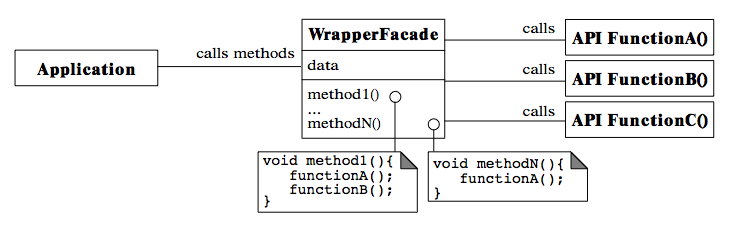
\includegraphics[width=12cm]{content/posa2/wrapper-facade/images/class-diagram.png}
	\caption{Wrapper Facade Klassendiagramm}
\end{figure}

Der Entwickler der Anwendung ruft eine Methode auf der Wrapper Facade auf, welche diesen Aufruf in einen oder mehrere System-API-Aufrufe umwandelt.


\subsection{Verwendung}

\begin{enumerate}
	\item \emph{Java}\\
	In Java gibt es beispielsweise Swing/AWT, um GUIs zu realisieren. Diese greifen schlussendlich auf das System-API zurück. Je nach Plattform kommt dafür eine andere Implementierung zum Einsatz.
\end{enumerate}


\subsection{Vorteile}

\begin{itemize}
	\item Ein einfaches, verständliches, konsistentes, robustes, objekt-orientiertes Interface für den plattformunabhängigen Zugriff auf low-level APIs. Dadurch erhöhte Wartbarkeit und Portierbarkeit.
\end{itemize}


\subsection{Nachteile}

\begin{itemize}
	\item Die Wrapper Facade stellt meistens nur den grössten gemeinsamen Nenner zur Verfügung: Also die Funktionalität, die sicher auf jeder Plattform verfügbar ist. Will man plattformspezifische Features nutzen, ist das nicht möglich. Indirektion bedeutet immer Overhead: Die Performance nimmt also ab.
\end{itemize}